%!TEX encoding = UTF-8 Unicode
%!TEX root = ../lect-week01.tex

%%%%%%%%%%%%%%%%%%%%%%%%%%%%%%%%%%%%%%

\Subsection{Att lära denna läsvecka \texttt{w01}}

\ifkompendium\else  %%%%%%%%%%%%%%%%%%%%%%%%%%%%%%%%%%%%%%%%%%%%%%%%%
\begin{Slide}{Att lära denna läsvecka \texttt{w01}}
%!TEX encoding = UTF-8 Unicode

    Modul \Emph{Introduktion}: Övn \Alert{\texttt{expressions}} $\rightarrow$ Labb \Alert{\texttt{kojo}}
    \begin{multicols}{3}\SlideFontTiny
    $\square$ sekvens \\
$\square$ alternativ \\
$\square$ repetition \\
$\square$ abstraktion \\
$\square$ editera \\
$\square$ kompilera \\
$\square$ exekvera \\
$\square$ datorns delar \\
$\square$ virtuell maskin \\
$\square$ litteral \\
$\square$ värde \\
$\square$ uttryck \\
$\square$ identifierare \\
$\square$ variabel \\
$\square$ typ \\
$\square$ tilldelning \\
$\square$ namn \\
$\square$ val \\
$\square$ var \\
$\square$ def \\
$\square$ definera och anropa funktion \\
$\square$ funktionshuvud \\
$\square$ funktionskropp \\
$\square$ procedur \\
$\square$ inbyggda grundtyper \\
$\square$ Int \\
$\square$ Long \\
$\square$ Short \\
$\square$ Double \\
$\square$ Float \\
$\square$ Byte \\
$\square$ Char \\
$\square$ String \\
$\square$ println \\
$\square$ typen Unit \\
$\square$ enhetsvärdet () \\
$\square$ stränginterpolatorn s \\
$\square$ if \\
$\square$ else \\
$\square$ true \\
$\square$ false \\
$\square$ MinValue \\
$\square$ MaxValue \\
$\square$ aritmetik \\
$\square$ slumptal \\
$\square$ math.random \\
$\square$ logiska uttryck \\
$\square$ de Morgans lagar \\
$\square$ while-sats \\
$\square$ for-sats \\
    \end{multicols}
    
\end{Slide}
\fi

\Subsection{Om programmering}

\ifkompendium\else
\SlideImg{Programming unplugged: Två frivilliga?}{../img/unplugged}
\SlideImg{Editera och exekvera ett program}{../img/kojo}
\fi

%%%

\ifkompendium\else
\SlideImg{Vad är en dator?}{../img/eniac}


\begin{Slide}{Hur fungerar en dator?}
\begin{tikzpicture}[node distance=2.0cm]
\node (input)  [startstop]               {Indata-enhet};
\node (cpu)    [process, below of=input] {CPU};
\node (output) [startstop,below of=cpu]  {Utdata-enhet};

\node (mem) [right of=cpu, xshift=4cm, draw = black, thick] {
\begin{minipage}{0.5\textwidth}\centering
\textbf{Minne} med minnesceller
\vspace{1em}

\begin{tabular}{|l | l|}
address & innehåll \\ \hline
0   & 42 \\ \hline
1   & 13 \\ \hline
2   & 18 \\ \hline
3   & 21 \\ \hline
4   & 55 \\ \hline
5   & 64 \\ \hline
6   & 48 \\ \hline 
... & ...
\end{tabular}
\end{minipage}
};

\draw [arrow] (input) -- (cpu);
\draw [arrow] (cpu) -- (output);
\draw [arrow] (cpu) -- (mem);
\draw [arrow] (mem) -- (cpu);

\node(memtext) [below of=mem, text width=7.0cm, scale=0.8, yshift=-1.5cm, xshift=0.5cm ] 
{Minnet innehåller endast \Alert{heltal} som \newline representerar \Emph{data} \Alert{och} \Emph{instruktioner}.};

%\node(memtext) [right of=input, text width=2cm, scale=0.8,xshift=1.0cm]{För\\människor};
%\node(output) [right of=output, text width=2cm, scale=0.8,xshift=1.0cm]{För\\maskiner};
\end{tikzpicture}
\end{Slide}

\fi

\begin{Slide}{Vad är programmering?}
\begin{itemize}
\item Programmering innebär att ge instruktioner till en maskin.
\item Ett \Emph{programmeringsspråk} används av människor för att skriva \Emph{källkod} som kan översättas av en \Emph{kompilator} till \Emph{maskinspråk} som i sin tur \Emph{exekveras} av en dator.
\end{itemize}


\begin{minipage}{.8\textwidth}
\begin{itemize}
\item Ada Lovelace skrev det första programmet redan på 1800-talet ämnat för en kugghjulsdator. 
\end{itemize}
\end{minipage}%
\begin{minipage}{.2\textwidth}
\centering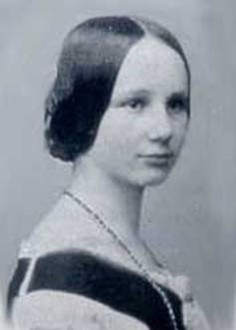
\includegraphics[width=0.6\columnwidth]{../img/ada}
\end{minipage}%
\begin{itemize}
\item \href{https://sv.wikipedia.org/wiki/Programmering}{sv.wikipedia.org/wiki/Programmering}
\item \href{https://en.wikipedia.org/wiki/Computer\_programming}{en.wikipedia.org/wiki/Computer\_programming}
\item Ha picknick i \href{http://kartor.lund.se/wiki/lundanamn/index.php/Ada_Lovelace-parken}{Ada Lovelace-parken} på Brunnshög!
\end{itemize}
\end{Slide}


\begin{Slide}{Vad är en kompilator?}
\begin{multicols}{2}
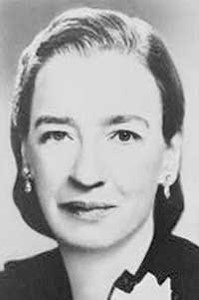
\includegraphics[width=0.8\columnwidth]{../img/grace}

\columnbreak %---------

Grace Hopper uppfann första kompilatorn 1952.\\
\href{https://en.wikipedia.org/wiki/Grace\_Hopper}{\SlideFontTiny en.wikipedia.org/wiki/Grace\_Hopper}
\vskip1em
%https://www.sharelatex.com/blog/2013/08/29/tikz-series-pt3.html
\begin{tikzpicture}[node distance=1.8cm]
\node (input) [startstop] {Källkod};
\node(inptext) [right of=input, text width=2cm, scale=0.8,xshift=1.0cm]{För\\människor};
\node (compile) [process, below of=input] {Kompilator};
\node (output) [startstop, below of=compile] {Maskinkod};
\node(outtext) [right of=output, text width=2cm, scale=0.8,xshift=1.0cm]{För\\maskiner};
\draw [arrow] (input) -- (compile);
\draw [arrow] (compile) -- (output);
\end{tikzpicture}
\end{multicols}
\end{Slide}


\ifkompendium\else

\begin{Slide}{Virtuell maskin (VM) == abstrakt hårdvara}
\begin{multicols}{2}

En VM är en ''dator'' implementerad i mjukvara som kan tolka en generell ''maskinkod'' som \Emph{översätts under körning} till den verkliga maskinens kod. \\
\vspace{1em}
Med en VM blir källkoden \Emph{plattformsoberoende} och fungerar på många olika maskiner. \\
\vspace{1em}
Exempel: \\ \Emph{Java Virtual Machine}
\columnbreak %---------

%https://www.sharelatex.com/blog/2013/08/29/tikz-series-pt3.html
\begin{tikzpicture}[node distance=1.4cm]
\node (input) [startstop] {Källkod};
\node (compile) [process, below of=input] {Kompilator};
\node (output) [startstop, below of=compile] {Generell ''maskinkod''};
\node (interp) [process, below of=output] {VM interpreterar};
\node (output2) [startstop, below of=interp] {Specifik maskinkod};
\draw [arrow] (input) -- (compile);
\draw [arrow] (compile) -- (output);
\draw [arrow] (output) -- (interp);
\draw [arrow] (interp) -- (output2);
\end{tikzpicture}
\end{multicols}
\end{Slide}
\fi

\begin{Slide}{Vad består ett program av?}
\begin{itemize}
\item Text som följer entydiga språkregler (gramatik): 
\begin{itemize}
\item \Emph{Syntax}: textens konkreta utseende 
\item \Emph{Semantik}: textens betydelse (vad maskinen gör/beräknar)
\end{itemize}
\item \Emph{Nyckelord}: ord med speciell betydelse, t.ex. \code{if}, \code{else}
\item \Emph{Deklarationer}: definitioner av nya ord: \code{def gurka = 42}
\item \Emph{Satser} är instruktioner som \emph{gör} något: \code{print("hej")} 
\item \Emph{Uttryck} är instruktioner som beräknar ett \emph{resultat}: \code{1 + 1}
\item \Emph{Data} är information som behandlas: t.ex. heltalet \code{42}
\item Instruktioner ordnas i kodstrukturer: (SARA)
\begin{itemize}
\item \Emph{Sekvens}: ordningen spelar roll för vad som händer
\item \Emph{Alternativ}: olika saker händer beroende på uttrycks värde
\item \Emph{Repetition}: satser upprepas många gånger
\item \Emph{Abstraktion}: nya byggblock skapas för att återanvändas
\end{itemize}
\end{itemize}
\end{Slide}

\begin{Slide}{Exempel på programmeringsspråk}
Det finns massor med olika språk och det kommer ständigt nya. 
\vspace{1em}
\begin{multicols}{2}
Exempel:
\begin{itemize}
\item Java
\item C
\item C++
\item C\#
\item Python
\item JavaScript
\item Scala
\end{itemize}

\columnbreak %---------

Topplistor:
\begin{itemize}
\item \href{http://www.tiobe.com/index.php/content/paperinfo/tpci/index.html}{TIOBE Index}
\item \href{http://pypl.github.io/PYPL.html}{PYPL Index}
\end{itemize}
\vspace{1em}

\includegraphics[width=0.8\columnwidth]{../img/pypl}
\end{multicols}

\end{Slide}


\begin{Slide}{Hello world}

\begin{REPLnonum}
scala> println("Hello World!")
Hello World!
\end{REPLnonum}

\begin{Code}
// this is Scala 

object Hello {
  def main(args: Array[String]): Unit = {
    println("Hejsan scala-appen!")
  }
}
\end{Code}


\begin{Code}[language=Java]
// this is Java 

public class Hi {
    public static void main(String[] args) {
        System.out.println("Hejsan Java-appen!");
    }
}
\end{Code}

\end{Slide}

\begin{Slide}{Utvecklingscykeln}
editera; kompilera; hitta fel och förbättringar; editera; kompilera; hitta fel och förbättringar; editera; kompilera; hitta fel och förbättringar; editera; kompilera; hitta fel och förbättringar; editera; kompilera; hitta fel och förbättringar; editera; kompilera; hitta fel och förbättringar; ...

\begin{Code}
upprepa(1000){
  editera
  kompilera
  testa
}
\end{Code}
\end{Slide}

\begin{Slide}{Utvecklingsverktyg}
\begin{itemize}
\item Din verktygskunskap är mycket viktig för din produktivitet. 
\item Lär dig kortkommandon för vanliga handgrep. 
\item Verktyg vi använder i kursen:
\begin{itemize}
\item Scala \Emph{REPL}: från övn 1
\item \Emph{Texteditor} för kod, t.ex \code{gedit} eller \code{atom}: från övn 2
\item Kompilera med \Emph{\code{scalac}} och \Emph{\code{javac}}: från övn 2
\item Integrerad utvecklingsmiljö (IDE)
\begin{itemize}
\item \Emph{Kojo}: från lab 1
\item \Emph{Eclipse+ScalaIDE} eller \Emph{IntelliJ IDEA} med Scala-plugin: från lab 3 i vecka 4
\end{itemize}
\item \Emph{jar} för att packa ihop och distribuera klassfiler
\item \Emph{javadoc} och \Emph{scaladoc} för dokumentation av kodbibliotek
\end{itemize}
\item Andra verktyg som är bra att lära sig:
\begin{itemize}
\item git för versionshantering
\item GitHub för kodlagring -- men \Alert{inte} av lösningar till labbar!
\end{itemize}
\end{itemize}
\end{Slide}


\ifkompendium\else  %%%%%%%%%%%%%%%%%%%%%%%%%%%%%%%%%%%%%%%%%%%%%%%%%

\begin{Slide}{Att skapa koden som styr världen}
\begin{multicols}{2}\footnotesize
I stort sett alla delar av samhället är beroende av programkod:
\begin{itemize}\scriptsize
\item kommunikation
\item transport
\item byggsektorn
\item statsförvaltning
\item finanssektorn
\item media \& underhållning
\item sjukvård
\item övervakning
\item integritet
\item upphovsrätt
\item miljö \& energi
\item sociala relationer
\item utbildning 
\item ...
\end{itemize}
\columnbreak %---------
Hur blir ditt framtida yrkesliv som systemutvecklare?
\begin{itemize}
\item  Det är sedan lång tid en skriande brist på utvecklare och bristen blir bara värre och värre... \\
  \href{http://computersweden.idg.se/2.2683/1.663879/oppen-kallkod-brist-kompetens}{CS 2016-08-23}
\item Störst brist är det på kvinnliga utvecklare: \\
\href{http://www.dn.se/ekonomi/it-branschen-hotas-av-brist-pa-kvinnor/}{DN 2015-04-02}
\item Global kompetensmarknad \\ 
  \href{http://computersweden.idg.se/2.2683/1.630901/det-finns-programmerare-och-sa-finns-det-programmerare}{CS 2015-06-14} \\
  \href{http://computersweden.idg.se/2.2683/1.662186/25-miljoner-utvecklare?queryText=miljoner\%20utvecklare}{CS 2016-07-14 }
\end{itemize}
\end{multicols}
\end{Slide}

\begin{Slide}{Utveckling av mjukvara i praktiken}
\begin{itemize}
\item \Emph{Inte bara kodning:} kravbeslut, releaseplanering, design, test, versionshantering, kontinuerlig integration, driftsättning, återkoppling från dagens användare, ekonomi \& investering, gissa om morgondagens användare, ... 
\item \Emph{Teamwork:} Inte ensamma hjältar utan autonoma team i decentraliserade organisationer med innovationsuppdrag
\item \Emph{Snabbhet:} Att koda innebär att hela tiden uppfinna nya ''byggstenar'' som ökar organisationens förmåga att snabbt skapa värde med hjälp av mjukvara. Öppen källkod. Skapa kraftfulla API:er.
\item \Emph{Livslångt lärande:} Lär nytt och dela med dig hela tiden. Exempel på pedagogisk utmaning: hjälp andra förstå och använda ditt API $\implies$ \textit{Samarbetskultur}
\end{itemize}
\end{Slide}


\fi %%%%%%%%%%%%%%%%%%%%%%%%%%%%%%%%%%%%%%%%%%%%%%%%%%%%


\Subsection{De enklaste beståndsdelarna: litteraler, uttryck, variabler}


\begin{Slide}{Literaler}
\begin{itemize}
\item Literaler representerar ett fixt \Emph{värde} i koden och används för att skapa \Alert{data} som programmet ska bearbeta.
\item Exempel: \\
\begin{tabular}{l l}
\code|42| & heltalslitteral\\
\code|42.0| & decimaltalslitteral\\
\code|'!'| & teckenlitteral, omgärdas med 'enkelfnuttar' \\
\code|"hej"| & stränglitteral, omgärdas med ''dubbelfnuttar'' \\
\code|true| & litteral för sanningsvärdet ''sant''\\
\end{tabular} 
\item Literaler har en \Emph{typ} som avgör vad man kan göra med dem.
\end{itemize}
\end{Slide}

\begin{Slide}{Exempel på inbyggda datatyper i Scala}
\begin{itemize}
\item Alla värden, uttryck och variabler har en \href{https://sv.wikipedia.org/wiki/Datatyp}{\Emph{datatyp}}, t.ex.: 
\begin{itemize}\footnotesize
\item \code{Int} för heltal 
\item \code{Long} för \textit{extra} stora heltal (tar mer minne)
\item \code{Double} för decimaltal, så kallade flyttal med flytande decimalpunkt
\item \code{String} för strängar
\end{itemize}
\item Kompilatorn håller reda på att uttryck kombineras på ett \Emph{typsäkert} sätt. Annars blir det kompileringsfel.
\item Scala och Java är s.k. \href{https://sv.wikipedia.org/wiki/Typsystem}{\Emph{statiskt typade}} språk, vilket innebär att all typinformation måste finnas redan vid kompileringsdags \Eng{compile time}\footnote{Andra språk, t.ex. Python och Javascript är dynamiskt typade och där skjuts typkontrollen upp till körningsdags \Eng{run time} \\ Vilka är för- och nackdelarna med statisk vs. dynamisk typning?}. 
\end{itemize}
\end{Slide}


\begin{Slide}{Grundtyper i Scala}\SlideFontSmall
Dessa \Emph{grundtyper} \Eng{basic types} finns inbyggda i Scala:

\begin{table}[H]
\renewcommand{\arraystretch}{1.4}
\begin{tabular}{p{0.24\textwidth}|p{0.21\textwidth}|l}
\textit{Svenskt namn} & \textit{Engelskt namn} & \Emph{Grundtyper} \\ \hline
heltalstyp & integral type & \texttt{Byte}, \texttt{Short}, \texttt{Int}, \texttt{Long}, \texttt{Char} \\
flyttalstyp  &  floating point \newline number types & \texttt{Float}, \texttt{Double} \\
numeriska typer & numeric types & heltalstyper och flyttalstyper \\
strängtyp \newline (teckensekvens) & string type & \texttt{String}  \\
sanningsvärdestyp  \newline (booelsk typ)& truth value type & \texttt{Boolean} \\
\end{tabular}
\end{table}

\end{Slide}

\begin{Slide}{Grundtypernas implementation i JVM}\SlideFontSmall
\begin{table}[H]
\renewcommand{\arraystretch}{1.4}
\begin{tabular}{l|l|l|l}
\Alert{Grundtyp} i &  Antal                &      Omfång&\Alert{primitiv typ} i\\
 \Emph{Scala} & bitar & minsta/största värde &\Emph{Java} \& \Emph{JVM}\\ \hline
\texttt{Byte}   &  8  & $-2^7$ ... $2^7-1$   & \texttt{byte} \\
\texttt{Short}  &  16 & $-2^{15}$ ... $2^{15}-1$ & \texttt{short} \\
\texttt{Char}   &  16 & $0$ ... $2^{16}-1$ & \texttt{char} \\
\texttt{Int}    &  32 & $-2^{15}$ ... $2^{15}-1$ & \texttt{int} \\
\texttt{Long}   &  64 & $-2^{15}$ ... $2^{15}-1$ & \texttt{long} \\
\texttt{Float}  &  32 & ± $3.4028235 \cdot 10^{38}$  & \texttt{float} \\
\texttt{Double} &  64 & ± $1.7976931348623157 \cdot 10^{308}$ & \texttt{double} \\
\end{tabular}
\end{table}

Grundtypen \texttt{String} lagras som en \emph{sekvens} av 16-bitars tecken av typen \texttt{Char} och kan vara av godtycklig längd (tills minnet tar slut).

\end{Slide}


\ifkompendium\else

\begin{Slide}{Uttryck}
\begin{itemize}
\item Ett \Emph{uttryck} består av en eller flera delar som blir en helhet. 
\item Delar i ett uttryck kan t.ex. vara: \\ literaler (42), operatorer (+), funktioner (sin), ... 
\item Exempel:
\begin{itemize}
\item Ett enkelt uttryck: \\ \code{42.0}
\item Sammansatta uttryck: \\
\code{40 + 2} \\
\code{(20 + 1) * 2} \\
\code{sin(0.5 * Pi)} \\
\code{"hej" + " på " + "dej"}
\end{itemize}

\item När programmet tolkas sker \Emph{evaluering} av uttrycket, vilket ger ett resultat i form av ett \Emph{värde} som har en \Emph{typ}.
\end{itemize}
\end{Slide}


\begin{Slide}{Variabler}\SlideFontSmall
\begin{itemize}
\item En \Emph{variabel} kan tilldelas värdet av ett enkelt eller sammansatt uttryck. 
\item En variabel har ett \Emph{variabelnamn}, vars utformning följer språkets regler för s.k. \Emph{identifierare}. 
\item En ny variabel införs i en \Emph{variabeldeklaration} och då den kan ges ett värde, \Emph{initialiseras}. Namnet användas som \Emph{referens} till värdet.
\item Exempel på variabeldeklarationer i Scala, notera \Emph{nyckelordet} \code{val}:
\begin{Code}
val a = 0.5 * Pi
val length = 42 * sin(a)
val exclamationMarks = "!!!"
val greetingSwedish = "Hej på dej" + exclamationMarks
\end{Code}

\item Vid exekveringen av programmet lagras variablernas värden i minnet och deras respektive värde hämtas ur minnet när de \Emph{refereras}. 

\item Variabler som deklareras med \code{val} kan endast tilldelas ett värde \Alert{en enda gång}, vid den initialisering som sker vid deklarationen. 
\end{itemize}

\end{Slide}


\begin{Slide}{Regler för identifierare}
\begin{itemize}
\item \Emph{Enkel} identifierare: t.ex. \code{gurka2tomat}
\begin{itemize}
\item Börja med bokstav
\item ...följt av bokstäver eller siffror
\item Kan även innehålla understreck
\end{itemize}

\item \Emph{Operator}-identifierare, t.ex. \code{+:}
\begin{itemize}
\item Börjar med ett operatortecken, t.ex. \code{+ - * / : ? ~ #}  
\item Kan följas av fler operatortecken
\end{itemize}

\item \Emph{Bokstavlig} identifierare: \code{`kan innehålla allt`}
\begin{itemize}
\item Börjar och slutar med \Emph{backticks}  \code{` `}  
\item Kan innehålla vad som helst (utom backticks)
\item Kan användas för att undvika krockar med reserverade ord: \texttt{\code{`}val\code{`}}
\end{itemize}

\item En identifierare får \Alert{inte} vara ett \Emph{reserverat ord}, se snabbreferensen för alla reserverade ord i Scala \& Java.
\end{itemize}
\end{Slide}



%\begin{Slide}{Regler för identifierare i Java}\footnotesize
%När kompilatorn ''läser''  \footnote{man säger ofta ''parsa'' i stället för ''läsa'' när kompilatorn tolkar koden} koden och och försöker hitta variabelnamn, antar den att du följer de entydiga syntaktiska reglerna för språket.  \\ \vskip1em För namn i Java gäller följande regler: %https://docs.oracle.com/javase/tutorial/java/nutsandbolts/variables.html
%\begin{itemize}
%\item Namn får inte vara \href{https://docs.oracle.com/javase/tutorial/java/nutsandbolts/_keywords.html}{reserverade ord}
%\item Stora och små bokstäver spelar roll \Eng{case sensistive} \\ \lstinline{int highScore;} och \lstinline{int highscore;} ger alltså två \textit{olika} variabler
%\item Namnet måste börja med en bokstav, ett understreck \_ eller ett dollartecken \$
%\item Namn får \textit{inte} innehålla blanktecken
%\item Namn får innehålla bokstäver, siffror, understreck \_ och dollartecken \$, men \textit{inte} andra specialtecken (alltså inte \lstinline~%&@!{(})/+-*~ etc.) 
%\end{itemize}
%\end{Slide}



\begin{Slide}{Att bygga strängar: konkatenering och interpolering}
\begin{itemize}
\item Man kan \Emph{konkatenera} strängar med operatorn + \\ \code{"hej" + " på " + "dej"}
\item Efter en sträng kan man konkatenera vilka uttryck som helst som då görs om till en sträng före konkateneringen: 
\begin{Code}
val x = 42
val msg = "Dubbla värdet av " + x + " är " + (x * 2) + "."
\end{Code}
\item Man kan i Scala (men inte Java) få hjälp av kompilatorn att övervaka bygget av strängar med \Emph{stränginterpolatorn} \Alert{s}:
\begin{Code}
val msg = s"Dubbla värdet av $x är ${x * 2}."
\end{Code}

\end{itemize}
\end{Slide}



\Subsection{Funktioner}

\begin{Slide}{Definiera funktioner}
\begin{itemize}
\item
\end{itemize}
\end{Slide}

\begin{Slide}{Paketet \texttt{scala.math}}
\begin{itemize}
\item math.random
\end{itemize}
\end{Slide}



\Subsection{Logik}

\begin{Slide}{Alternativ med if-uttryck}
\begin{itemize}
\item
\end{itemize}
\end{Slide}


\begin{Slide}{Logiska uttryck}
\begin{itemize}
\item
\end{itemize}
\end{Slide}

\begin{Slide}{de Morgans lagar}
\begin{itemize}
\item
\end{itemize}
\end{Slide}

\Subsection{Satser}




%%%%%%%%%%%%%%%%%%%%%%%%
\begin{Slide}{Tilldelningssatser}\scriptsize

Vad är egentligen en variabel?
\begin{itemize}
\item En variabel har ett \Emph{namn} och kan lagra ett \Emph{värde} av en viss \Emph{typ}
\item Variabler måste  \Emph{deklareras} och då får kompilatorn reda på vilket namnet är och vilken typ av värden som variabeln kan lagra: \\ \lstinline{int x; }
\item När variabler deklareras är det oftast bäst att direkt ge dem ett initialvärde:  \\ \lstinline{int x = 42; }
\item En variabeldeklaration medför att plats i datorns minne reserveras. \\Vi ritar detta såhär: \\ 
\begin{tikzpicture}[]
\matrix [matrix of nodes, row sep=0, column 2/.style={nodes={rectangle,draw,minimum width=3em}}]
{
x   & 42 \\
};
\end{tikzpicture}
\end{itemize}

\begin{columns}
\begin{column}{0.3\textwidth}
Dessa deklarationer...
\begin{lstlisting}
int x = 42;    
int y = x + 1;   
\end{lstlisting}
\end{column}
\begin{column}{0.5\textwidth}
... ger detta innehåll någonstans i minnet:

%http://tex.stackexchange.com/questions/18521/tikz-matrix-as-a-replacement-for-tabular
\begin{tikzpicture}[]
\matrix [matrix of nodes, row sep=0, column 2/.style={nodes={rectangle,draw,minimum width=3em}}]
{
x   & 42 \\
y   & 43 \\
};
\end{tikzpicture}
\end{column}
\end{columns}
\end{Slide}


\begin{Slide}{Vad händer egentligen vid en tilldelning?}\footnotesize
\begin{itemize}
\item Med en \Emph{tilldelningssats} kan vi ge en tidigare deklarerad variabel ett nytt värde: 
\begin{lstlisting} 
x = 1;
\end{lstlisting}
\item Det gamla värdet försvinner för alltid och det nya värdet lagras istället:
\begin{tikzpicture}[]
\matrix [matrix of nodes, row sep=0, column 2/.style={nodes={rectangle,draw,minimum width=3em}}]
{
x   & 1 \\
};
\end{tikzpicture}
\item Likhetstecknet används alltså för att \textit{ändra} variablers värden och det är ju \textit{inte} samma sak som matematisk likhet \footnote{\scriptsize Arv från C, Fortran mfl. I \href{https://en.wikipedia.org/wiki/Assignment_\%28computer_science\%29}{andra språk} används  t.ex. \lstinline{x := 42} eller \lstinline{x <- 42}}. Vi kan till exempel skriva denna tilldelningssats:
\begin{lstlisting} 
x = x + 1;   //Vad händer här?
\end{lstlisting}
\end{itemize}
\end{Slide}

\begin{Slide}{Övning: Tilldelningar i sekvens}\footnotesize
\begin{columns}
\begin{column}{0.33\textwidth}
Rita hur minnet ser ut efter varje rad nedan:
\vskip1em
\begin{lstlisting}[ numbers=left,]
int u, x, y, z;
x = 10;
y = 2 * x + 1;
z = (y + x) + (y - x);
x = x + 1;
\end{lstlisting}
\end{column}
\begin{column}{0.6\textwidth}

\scriptsize En variabel som ännu inte initierats har ett odefinierat värde, anges nedan med frågetecken.
\begin{table}[] 
\centering\scriptsize
%http://tex.stackexchange.com/questions/83930/what-are-the-different-kinds-of-boxes-in-latex
\newcommand{\mybox}[1]{\raisebox{-0.5mm}{\framebox(21,14){#1}}\vspace{0.5mm}}
\begin{tabular}{cccccc}
 & rad 1 & rad 2 & rad 3 & rad 4  & rad 5\\ 
u& \mybox{? } &  \mybox{}   &   \mybox{}   & \mybox{} & \mybox{} \\
x& \mybox{? } &  \mybox{}   &   \mybox{}   & \mybox{} & \mybox{} \\
y& \mybox{? } &  \mybox{}   &   \mybox{}   & \mybox{} & \mybox{} \\
z& \mybox{? } &  \mybox{}   &   \mybox{}   & \mybox{} & \mybox{} \\
\end{tabular}
\end{table}

\end{column}
\end{columns}
\end{Slide}

\begin{Slide}{Förkortade tilldelningssatser}
\begin{itemize}
\item
\end{itemize}
Förkortade tilldelningssatser

\end{Slide}

\begin{Slide}{Variabler som ändrar värden kan vara knepiga}
\begin{itemize}
\item Variabler som \Alert{förändras} över tid kan vara svåra att resonera kring.

\item Många buggar beror på att variabler förändras på felaktiga och oanade sätt.

\item Föränderliga värden blir speciellt svåra i kod som körs jämlöpande (parallelt). 

\item I produktionskod används därför \code{val} överallt där det går och \code{var} bara om det verkligen behövs.
\end{itemize}
\end{Slide}
%%%%%%%%%%



\begin{Slide}{Kontrollstrukturer}
Används för att kontrollera (förändra) sekvensen.
\begin{itemize}
\item if-sats
\item while-sats
\item for-sats
\end{itemize}
\end{Slide}

\begin{Slide}{if-sats}
\begin{itemize}
\item
\end{itemize}
\end{Slide}

\begin{Slide}{while-sats}
\begin{itemize}
\item
\end{itemize}
\end{Slide}

\begin{Slide}{for-sats}
\begin{itemize}
\item
\end{itemize}
\end{Slide}

\begin{Slide}{Procedurer}
println
\begin{itemize}
\item
\end{itemize}
\end{Slide}


\begin{Slide}{Om veckans övning: \code{expressions}}
\begin{itemize}
\item
\end{itemize}
\end{Slide}

\begin{Slide}{Om veckans labb: \code{kojo}}
\begin{itemize}
\item
\end{itemize}
\end{Slide}


\fi



%%%%%%%%%%%%%%%%%%%%%%%%%%%%%%%%%%%%%% nedan redan meddelat i introveckan
%\ifkompendium\else
%\Subsection{Meddelande från \href{http://lth.se/code}{Code@LTH}} 
%\fi